% !TEX root = main.tex
\subsection{J-Kopplung zur chemischen Strukturanalyse}
Eine weitere Anwendung der NMR-Technologie stellt die Möglichkeit dar chemische Strukturen zu analysieren.
Im vorliegenden Beispiel soll dabei Difluorobenzene untersucht werden.
Dabei wird die Verbindung zum einen auf die Kopplungskostante zwischen den einzelnen Flour- und Wasserstoffatomen analysiert, dabei kann ermittelt werden, ob schwache Kopplung vorliegt zudem sollen auch Verhältnisse der Peakgrößen betrachtet werden.
Zunächst sollen daher einige grundlegende Zusammenhänge erläutert werden.
Da es sich bei dem vorliegenden Molekül um eine hetero-nukleare Verbindung zwischen Fluor (\ce{^19F}) und Wasserstoff (\ce{^1H}) handelt und der Versuchsaufbau während des Experiments auf die Larmorfrequenz von Wasserstoff ($\omega_{\text{L,H}} = \SI{1839}{\per \second}$) ausgerichtet ist müssen zunächst justierungen vorgenommen werden.
Dabei kann nach
\begin{align}
    \omega = \gamma \cdot B , \label{eq: LarmorB}    
\end{align}
die Larmorfrequenz für Fluor ($\omega_{\text{L,F}} = \SI{1730}{\per \second}$) berechnet werden. 
Die gyromagnetischen Verhältnisse $\gamma$ von Wasserstoff ($\gamma = \SI{2.675 e8}{\per \second \per \tesla}$) und Fluor ($\gamma = \SI{2.517 e8}{\per \second \per \tesla}$) wurden dabei \cite{Schmidt} entnommen. 
Das anliegende B-Feld war aus dem bis dato verwendeten Setups bekannt.
Anschließend wurde abermals nach Formel \eqref{eq: larmorcalc} die Kapazität des Schwingkreises ermittelt und ebenfalls auf die Larmorfrequenz abgestimmt.
Somit konnte ein Spektrum für Fluor angezeigt und die entsprechenden Parameter weiter optimiert werden. \cite{Schmidt} \\
Um anschließend beide Elemente gleichermaßen abbilden zu können, wurde sowohl der Mittelwert der Larmorfrequenzen ($\omega_{\text{L,MW}} = \SI{1787}{\per \second}$) wie auch der Kapazitäten ($C_{\text{MW}} = \SI{14.7}{\nano \farad}$) eingestellt und damit eine ,,Pulse and Collect''-Messung durchgeführt.

Dabei soll zunächst erläutert werden, welche Erkentnisse aus dem gewonnen Spektrum gewonnen werden können und welche Ergebnisse zu erwarten sind.


Abbildung \ref{fig:JKSchema} zeigt schematisch ein zu erwartendes Spektrum entnommen aus \cite{Schmidt}.
\begin{figure}[H]
    \centering
    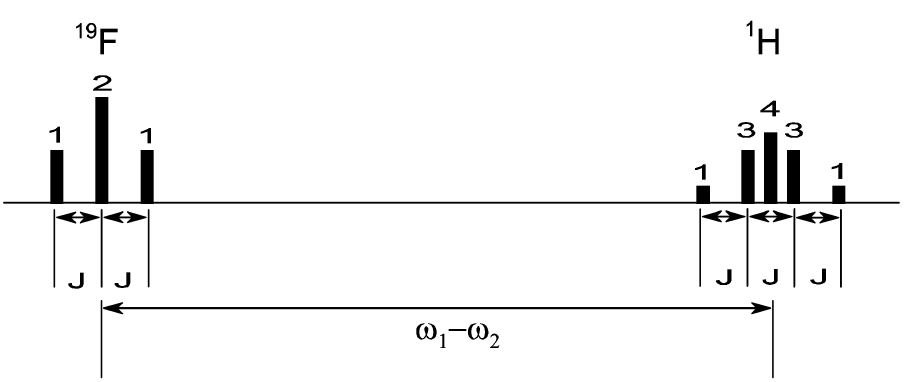
\includegraphics[width= 0.75\textwidth]{Abbildungen/JKopplungSchema.png} 
    \caption[Schematische Darstellung eines Spektrums zur veranschaulichung der erwartbaren Ergebnisse durch die Analyse der J-Kopplung.]{Die Abbildung zeigt schematisch ein Spektrum für Trifluoroethanol.
    Dabei ist zu erkennen, welche Erkentnisse aus dem Spektrum abgelesen werden können.
    Diese sind zum einen die Kopplungskostante $J$, welche als Abstand zwischen den Peaks eines Elements verstanden wird, zum anderen kann die Annahme der schwachen Kopplung nach Formel \eqref{eq:SchwacheKopplung} überprüft werden.
    Zudem kann aus dem Verhältnis der Peakintegrale die Verteilung der Intensitäten berechnet werden.
    Diese folgt abhängig der Anzahl auftretender Maxima dem \textsc{Pascal}'schen Dreieck.}
    \label{fig:JKSchema}
\end{figure}

Hierbei ist allerdings ein anderes Molekül, Trifluoroethanol, veranschaulicht.
Erkennbar ist, dass aus dem Abstand der einzelnen Peakmaxima bei Fluor und Wasserstoff die Kopplungskonstante $J$ bestimmt werden kann.
Im Falle schwacher Kopplung gilt zudem die Relation
\begin{align}
    2 \pi \cdot J \ll \vert \omega_1 - \omega_2 \vert , \label{eq:SchwacheKopplung}
\end{align}
zwischen Kopplungskonstante $J$ und dem Abstand der Hauptmaxima $\vert \omega_1 - \omega_2 \vert$ der beiden Elemente.
Hierbei wird angenommen, dass bei der \textsc{Zeeman}-Wechselwirkung lediglich ein Störterm erster Ordnung durch die J-Kopplung berücksichtigt werden muss.
Sollten Störungen höherer Ordnung aufgrund stärkerer Kopplung vorliegen, so können diese die Peakbreite beeinflussen und vergrößern.
Zuletzt ist die Verteilung der Peakintensitäten, beziehungsweise das Verhältnis derer zueinander dargestellt.
Diese folgen je nach Anzahl der vorliegenden Peaks pro Element einer Verteilung nach dem \textsc{Pascal}'schen Dreieck.
Ermittelt wird diese Verteilung durch die Integration über die Peaks.
Die Anzahl vorliegender Peaks ist dadurch bestimmt wieviele Spins pro Element zur Wechselwirkung beitragen.
Hat ein Element $N$ Spins, so spaltet das andere Element in $N+1$ Peaks auf.
Entsprechend sind im vorliegenden Molekül je drei Maxima pro Element zu erwarten. 

Abbildung \ref{fig:JKopplungExp} zeigt das am Versuchstag gewonnene Spektrum.
Hierbei sind farbig (blau für Fluor und grün für Wasserstoff) die jeweils drei \textsc{Gauss}-Fits zu erkennen. 
Bei \SI{1750}{\hertz} ist zudem ein Peak zu erkennen, welcher wie bereits beschrieben auf die Taktung der deutschen Netzspannung zurückzuführen ist.

\begin{figure}[H]
    \centering
    % GNUPLOT: LaTeX picture with Postscript
\begingroup
  % Encoding inside the plot.  In the header of your document, this encoding
  % should to defined, e.g., by using
  % \usepackage[cp1252,<other encodings>]{inputenc}
  \inputencoding{cp1252}%
  \makeatletter
  \providecommand\color[2][]{%
    \GenericError{(gnuplot) \space\space\space\@spaces}{%
      Package color not loaded in conjunction with
      terminal option `colourtext'%
    }{See the gnuplot documentation for explanation.%
    }{Either use 'blacktext' in gnuplot or load the package
      color.sty in LaTeX.}%
    \renewcommand\color[2][]{}%
  }%
  \providecommand\includegraphics[2][]{%
    \GenericError{(gnuplot) \space\space\space\@spaces}{%
      Package graphicx or graphics not loaded%
    }{See the gnuplot documentation for explanation.%
    }{The gnuplot epslatex terminal needs graphicx.sty or graphics.sty.}%
    \renewcommand\includegraphics[2][]{}%
  }%
  \providecommand\rotatebox[2]{#2}%
  \@ifundefined{ifGPcolor}{%
    \newif\ifGPcolor
    \GPcolorfalse
  }{}%
  \@ifundefined{ifGPblacktext}{%
    \newif\ifGPblacktext
    \GPblacktexttrue
  }{}%
  % define a \g@addto@macro without @ in the name:
  \let\gplgaddtomacro\g@addto@macro
  % define empty templates for all commands taking text:
  \gdef\gplbacktext{}%
  \gdef\gplfronttext{}%
  \makeatother
  \ifGPblacktext
    % no textcolor at all
    \def\colorrgb#1{}%
    \def\colorgray#1{}%
  \else
    % gray or color?
    \ifGPcolor
      \def\colorrgb#1{\color[rgb]{#1}}%
      \def\colorgray#1{\color[gray]{#1}}%
      \expandafter\def\csname LTw\endcsname{\color{white}}%
      \expandafter\def\csname LTb\endcsname{\color{black}}%
      \expandafter\def\csname LTa\endcsname{\color{black}}%
      \expandafter\def\csname LT0\endcsname{\color[rgb]{1,0,0}}%
      \expandafter\def\csname LT1\endcsname{\color[rgb]{0,1,0}}%
      \expandafter\def\csname LT2\endcsname{\color[rgb]{0,0,1}}%
      \expandafter\def\csname LT3\endcsname{\color[rgb]{1,0,1}}%
      \expandafter\def\csname LT4\endcsname{\color[rgb]{0,1,1}}%
      \expandafter\def\csname LT5\endcsname{\color[rgb]{1,1,0}}%
      \expandafter\def\csname LT6\endcsname{\color[rgb]{0,0,0}}%
      \expandafter\def\csname LT7\endcsname{\color[rgb]{1,0.3,0}}%
      \expandafter\def\csname LT8\endcsname{\color[rgb]{0.5,0.5,0.5}}%
    \else
      % gray
      \def\colorrgb#1{\color{black}}%
      \def\colorgray#1{\color[gray]{#1}}%
      \expandafter\def\csname LTw\endcsname{\color{white}}%
      \expandafter\def\csname LTb\endcsname{\color{black}}%
      \expandafter\def\csname LTa\endcsname{\color{black}}%
      \expandafter\def\csname LT0\endcsname{\color{black}}%
      \expandafter\def\csname LT1\endcsname{\color{black}}%
      \expandafter\def\csname LT2\endcsname{\color{black}}%
      \expandafter\def\csname LT3\endcsname{\color{black}}%
      \expandafter\def\csname LT4\endcsname{\color{black}}%
      \expandafter\def\csname LT5\endcsname{\color{black}}%
      \expandafter\def\csname LT6\endcsname{\color{black}}%
      \expandafter\def\csname LT7\endcsname{\color{black}}%
      \expandafter\def\csname LT8\endcsname{\color{black}}%
    \fi
  \fi
    \setlength{\unitlength}{0.0500bp}%
    \ifx\gptboxheight\undefined%
      \newlength{\gptboxheight}%
      \newlength{\gptboxwidth}%
      \newsavebox{\gptboxtext}%
    \fi%
    \setlength{\fboxrule}{0.5pt}%
    \setlength{\fboxsep}{1pt}%
\begin{picture}(7200.00,5040.00)%
    \gplgaddtomacro\gplbacktext{%
      \csname LTb\endcsname%%
      \put(814,704){\makebox(0,0)[r]{\strut{}$0$}}%
      \put(814,1218){\makebox(0,0)[r]{\strut{}$0.5$}}%
      \put(814,1733){\makebox(0,0)[r]{\strut{}$1$}}%
      \put(814,2247){\makebox(0,0)[r]{\strut{}$1.5$}}%
      \put(814,2762){\makebox(0,0)[r]{\strut{}$2$}}%
      \put(814,3276){\makebox(0,0)[r]{\strut{}$2.5$}}%
      \put(814,3790){\makebox(0,0)[r]{\strut{}$3$}}%
      \put(814,4305){\makebox(0,0)[r]{\strut{}$3.5$}}%
      \put(814,4819){\makebox(0,0)[r]{\strut{}$4$}}%
      \put(946,484){\makebox(0,0){\strut{}$1700$}}%
      \put(2410,484){\makebox(0,0){\strut{}$1750$}}%
      \put(3875,484){\makebox(0,0){\strut{}$1800$}}%
      \put(5339,484){\makebox(0,0){\strut{}$1850$}}%
      \put(6803,484){\makebox(0,0){\strut{}$1900$}}%
    }%
    \gplgaddtomacro\gplfronttext{%
      \csname LTb\endcsname%%
      \put(308,2761){\rotatebox{-270}{\makebox(0,0){\strut{}Amplitude in $\si{\milli \second}$}}}%
      \put(3874,154){\makebox(0,0){\strut{}Frequenz in $\si{\hertz}$}}%
      \csname LTb\endcsname%%
      \put(5816,4646){\makebox(0,0)[r]{\strut{}Messung zur J-Kopplung}}%
      \csname LTb\endcsname%%
      \put(5816,4426){\makebox(0,0)[r]{\strut{}\textsc{Lorentz}-Fit}}%
    }%
    \gplbacktext
    \put(0,0){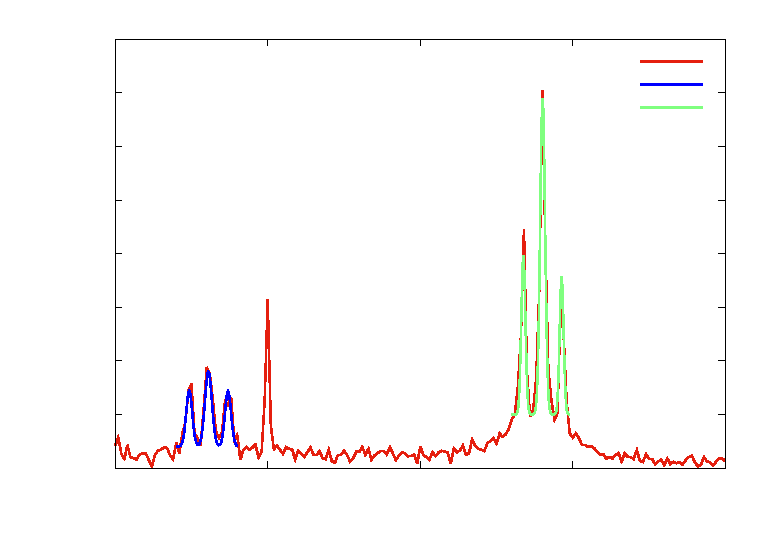
\includegraphics{plots/JKopplung}}%
    \gplfronttext
  \end{picture}%
\endgroup

    \caption{TODO!!;\\
    Zum tunen benutzte Daten des Puls and collect Experiments; Man soll noch die Integrale berechnen der einzelnen Peaks(aus den Integralen bekommt man dann das Verhältnuis von 1:2:3:3:2:1 oder so halt); Diese Peaks fitten bzw den abstand der Maximas berechnen=< daraus dann die Kopplungaskostante}
    \label{fig:JKopplungExp}
\end{figure}

Durch die \textsc{Gauss}-Fits konnten sowohl die Lage der Maxima, die Peakbreiten sowie die Integrale der Peaks berechnet werden.
Dabei wurde zudem die jeweilige Standardabweichung $\sigma$ als ein Fitparameter gewonnen, welche in Folge als Unsicherheit der Peakposition verwendet wurde.
Die Integrale der Peaks konnten dabei dadurch berechnet werden, dass das \textsc{Gauss}-Integral 
\begin{align}
    skbd
\end{align}
auf $1$ normiert ist
